\documentclass[a4paper]{scrartcl}

% Font and Language
\usepackage[utf8]{inputenc}
\usepackage[T1]{fontenc}
\usepackage[english]{babel}
\usepackage{lmodern}
\usepackage[hidelinks]{hyperref}


% Do not change font size, parskip or margin.
%Attempts to make a shorter paper appear larger will lead to course failure.
\KOMAoptions{fontsize=12pt}
\KOMAoptions{parskip=off}

\usepackage[
	left=2.5cm,
	right=2.5cm,
	top=2.5cm,
	bottom=4.5cm
]{geometry}

% Bibliography
\usepackage[backend=biber]{biblatex}
\usepackage{csquotes}
\addbibresource{references.bib}

% Add blindtext
\usepackage{blindtext}

% Running heads and foots
\usepackage[headsepline,footsepline]{scrlayer-scrpage}

% Set title

\newcommand{\paperTitle}{ComfortSphere: A Smart Home System for\\ Indoor Environment Optimization}
\title{\paperTitle}
\clearpairofpagestyles
\rehead{\paperTitle}
\rohead{\paperTitle}

% Set your name, your mail and matrikel number
\newcommand{\paperAuthor}{Joshi Juhi Ramesh, Amardeep Mishra,\\ Hardikkumar Savaliya, Mohammad Sheikh,\\ Hammad Chaudhary}
\author{
    Juhi Joshi~<jr.joshi@stud.fh-sm.de>, 316800\\
    Amardeep Mishra~<a.mishra@stud.fh-sm.de>, 316652\\
    Hardikkumar Savaliya~<hv.savaliya@stud.fh-sm.de>, 313904\\
    Mohammad Sheikh~<mzi.sheikh@stud.fh-sm.de>, 312538\\
    Hammad Chaudhary<rehman@stud.fh-sm.de>, 313955
    }

\lehead{\paperAuthor}
\lohead{\paperAuthor}




% Set page numbering
\usepackage{lastpage}
\refoot{\thepage{}of\pageref{LastPage}}
\rofoot{\thepage{}of\pageref{LastPage}}

% Add suas logo
\usepackage{graphicx}
\KOMAoptions{footheight=3cm}
\lefoot{\vspace*{1.5 in}
\includegraphics[height=1cm]{suas-logo}}
\lofoot{
\includegraphics[height=2cm]{suas-logo}}
\cfoot{\href{https://github.com/hardik2108/documentation}{\textbf{GitHub Repository}}}

% Do not show date
\date{}

\begin{document}
	\maketitle
	
 	\section{Abstract}
		{ComfortSphere revolutionizes modern living by seamlessly integrating IoT-enabled household appliances into an intelligent, responsive system. By utilizing advanced motion sensors, it automatically adjusts lighting, heating, and humidifiers to create a living environment tailored to individual needs and preferences. The accompanying webapp provides users with a simple and intuitive way to monitor and customize their settings, ensuring that every room feels just right. Whether it's adjusting the temperature on a chilly evening, fine-tuning humidity levels, or optimizing lighting based on activity, ComfortSphere takes care of the details so users can focus on what matters most. Designed for convenience and adaptability, ComfortSphere transforms ordinary living spaces into dynamic environments that respond effortlessly to the rhythms of daily life.}

	\section{Introduction}
\label{sec:intro}

The IoT-supported smart home market is rapidly expanding, with applications ranging from simple remote controls to advanced automated ecosystems. Modern smart home solutions aim to enhance energy efficiency, security, and user convenience by integrating intelligent sensors and automation technologies. \textbf{ComfortSphere} leads this innovation with a customizable smart room system that ensures seamless indoor climate control. Designed for versatility, it is suitable for homes, hospitals, and workplaces, providing optimal comfort and convenience while minimizing energy waste.

ComfortSphere utilizes advanced sensor technology and real-time data analytics to automatically adjust environmental parameters such as temperature, humidity, lighting, and occupancy-based settings. By leveraging IoT connectivity, it enables remote monitoring and control, allowing users to personalize their indoor environment through a user-friendly interface. The system continuously learns user preferences and adapts accordingly, enhancing overall efficiency.

Key components of the ComfortSphere system include:

\begin{itemize}
\item \textbf{DHT22 sensor}: Provides accurate temperature and humidity readings to maintain optimal indoor air quality.
\item \textbf{HC-SR501 PIR sensor}: Detects motion and occupancy to adjust climate and lighting settings dynamically, improving energy efficiency.
\item \textbf{TSL2561 sensor}: Measures ambient light intensity, enabling precise lighting adjustments for comfort and energy savings.
\end{itemize}

At the core of the system is the \textbf{Pinecone microcontroller}, which ensures smooth data processing, real-time responsiveness, and seamless communication between sensors and control mechanisms. This microcontroller enables the integration of machine learning algorithms for predictive analytics, allowing the system to anticipate user needs and preemptively adjust settings for an enhanced experience.

With its modular architecture, ComfortSphere is designed to be easily expandable, supporting additional IoT devices and sensors as needed. Its compatibility with voice assistants and mobile applications further enhances user accessibility, making smart home management effortless.

By combining automation, artificial intelligence, and IoT connectivity, ComfortSphere redefines indoor climate control, delivering a seamless and intelligent living experience.

	\subsection*{Use Cases}
	\begin{itemize}
		\item \textbf{Personal Use}: ComfortSphere customizes environments for relaxation, work, and sleep while optimizing energy usage in unoccupied spaces to enhance eco-friendliness.
		\item \textbf{Specialized Environments}: In hospitals and care facilities, ComfortSphere maintains precise climate conditions to support patients with respiratory needs, ensuring health and safety.
	\end{itemize}

	By integrating advanced sensors with user-defined settings, ComfortSphere enhances comfort, promotes health, and fosters sustainable living.
    
    \subsection{Problem Statement}
    Despite significant advances in smart home technology, many existing indoor climate control systems remain inflexible, energy-inefficient, and insensitive to users' health requirements. Traditional climate control systems often operate on fixed schedules, leading to suboptimal comfort levels and unnecessary energy consumption. Additionally, current solutions rarely address the specific needs of individuals with respiratory conditions or other health concerns that require precise environmental control.
    
    Furthermore, existing systems typically compartmentalize different aspects of the indoor environment—treating temperature, humidity, lighting, and air quality as separate domains rather than as interconnected elements that collectively determine user comfort and wellbeing. This fragmented approach results in suboptimal environmental conditions and fails to leverage the potential synergies between these elements.
    
    \subsection{Research Objectives}
    This research aims to address these challenges through the development and evaluation of ComfortSphere, an integrated smart home system that optimizes indoor environmental conditions. Specifically, the study addresses the following objectives:
    
    \begin{itemize}
        \item To design and implement an IoT-based system that seamlessly integrates temperature, humidity, and lighting control based on real-time sensor data.
        \item To develop adaptive algorithms that adjust environmental parameters based on occupancy detection, enhancing both comfort and energy efficiency.
        \item To evaluate the system's performance across different user groups, with a particular focus on individuals with specific health needs.
        \item To assess energy savings and sustainability benefits achieved through motion-based climate control.
        \item To develop a user-friendly interface that allows for easy monitoring and customization of environmental settings.
    \end{itemize}
    
    \subsection{Significance of Research}
    This research contributes to the evolving field of smart home technology in several key ways. First, it offers a holistic approach to indoor climate control by integrating multiple environmental factors into a cohesive system. Second, it addresses the specific needs of users with health concerns, an aspect often overlooked in existing solutions. Third, it incorporates energy efficiency as a core design principle, aligning with global sustainability goals.
    
    The significance of this research extends beyond technical innovation to include social impact. By creating environments that support health and wellbeing, ComfortSphere has the potential to improve quality of life, particularly for vulnerable populations such as the elderly or those with chronic respiratory conditions. Additionally, the energy-saving features of the system contribute to broader environmental sustainability efforts.
    
    Furthermore, this research lays the groundwork for future developments in adaptive indoor environments, potentially informing the design of next-generation smart buildings and healthcare facilities. The insights gained from this study will help bridge the gap between technological capability and user-centered design in smart home systems.

	\section{Literature Review}
	\label{sec:Literature Review}
	The literature review on IoT-enabled smart home systems highlights the significant potential these technologies have in addressing a wide range of environmental and energy-related challenges. Research in this area has shown that the efficient control of indoor climate, particularly through the regulation of temperature and humidity, plays a crucial role in enhancing the comfort and health of users. However, many existing solutions primarily focus on energy efficiency and automation, often overlooking the integration of health-related metrics. This creates a gap in addressing the specific needs of users who have respiratory sensitivities or other health concerns. \textbf{Comfort-Sphere} aims to fill this gap by embedding features into its design that specifically respond to the health-oriented needs of users, ensuring not only comfort but also improved well-being.

	\subsection{Humidity-Based Temperature Control}
	In the study \cite{paper1} titled \textit{"Humidity-Based Automated Room Temperature Controller Using IoT"}, the authors proposed a humidity-based automated temperature control system using an electric heater to maintain desired climate conditions. Although effective in maintaining temperature and humidity levels, the system does not account for health-specific metrics or energy efficiency. Comfort-Sphere addresses these limitations by incorporating advanced sensors, such as the DHT22 sensor, which offers higher precision, and integrating it with health-oriented features, such as real-time monitoring and automatic adjustments for individuals with specific respiratory needs.

	\subsection{Energy Efficiency in Smart Buildings through IoT Approaches}
	Metallidou et al. \cite{paper2} explore the application of IoT technologies to create energy-efficient smart building systems. They emphasize the role of low-cost IAQ sensors in enabling intelligent ventilation systems that operate based on real-time pollutant levels rather than fixed schedules. Such systems provide substantial energy savings by ensuring ventilation systems only run when necessary. Comfort-Sphere takes this a step further by integrating motion detection, ensuring that the climate control system adapts to occupancy. This adaptive system minimizes energy consumption by reducing unnecessary climate adjustments in unoccupied spaces, leading to more efficient energy use while maintaining a comfortable and healthy environment.

	\subsection{A Review of IoT Applications in Smart Home Automation}
	In \cite{paper3}, Sepasgozar et al. provided an extensive review of IoT and AI applications in smart home automation. They focused on the integration of AI, renewable energy, and environmental sensors to enhance energy efficiency and improve indoor air quality. The paper highlights the importance of integrating solar energy in powering HVAC systems, making ventilation and air quality management more cost-effective and environmentally friendly. However, many of the systems discussed in this paper focus primarily on monitoring rather than actively controlling indoor environments. Comfort-Sphere overcomes this limitation by offering automated, real-time climate control, allowing for a more dynamic and personalized approach to both comfort and health management. The integration of motion sensors ensures that Comfort-Sphere only adjusts climate settings when users are present, maximizing energy savings while offering a tailored environment.

	\subsection{Portable Humidity and Temperature Monitoring Nodes}
	In \cite{paper4}, the study \textit{"A Portable Node of Humidity and Temperature Sensor for Indoor Environment Monitoring"} describes a compact, portable system designed for monitoring indoor environments using a DHT11 sensor, a Zigbee module, and an STM32L100 microcontroller. While the system's portability and low power consumption are beneficial for basic monitoring, it lacks the ability to automatically adjust climate settings or address health-related needs. Comfort-Sphere advances this by using the DHT22 sensor, which provides higher accuracy in temperature and humidity readings. Moreover, Comfort-Sphere integrates motion sensing, allowing for adaptive, energy-efficient climate control. This enables the system to not only monitor but also adjust the indoor environment to support health-specific needs, such as maintaining consistent humidity levels for respiratory comfort.

	\subsection{Intelligent Indoor Temperature and Humidity Control}
	In \cite{paper5}, the authors present an \textit{"Intelligent Indoor Temperature and Humidity Control System"} that uses wireless communication and control algorithms to regulate temperature and humidity levels. The system's ability to wirelessly communicate with HVAC components such as air conditioners and humidifiers allows for real-time adjustments, enhancing user comfort. However, this system does not incorporate real-time health-based calibrations or personalized climate adjustments for users with specific health concerns. Comfort-Sphere goes beyond this by using dynamic optimization to personalize climate adjustments based on user-defined health needs, such as those of individuals suffering from asthma or COPD. This level of customization ensures that the system not only maintains optimal comfort but also contributes to the user's health and well-being by creating an environment that supports respiratory health.

    \subsection{Machine Learning for Smart Home Environment Control}
    The application of machine learning in smart home systems has gained significant traction in recent years. Minoli et al. \cite{paper6} explore how IoT-based smart home systems can leverage machine learning algorithms to adapt to user preferences and behaviors over time. Their research demonstrates that by analyzing patterns in user behavior, systems can predict and preemptively adjust environmental settings, leading to enhanced comfort and reduced manual intervention. ComfortSphere builds upon this foundation by incorporating a learning component that adapts to individual user preferences, creating a personalized experience that evolves over time. Unlike many existing systems that rely solely on preset configurations, ComfortSphere's adaptive approach ensures that the indoor environment continuously aligns with user needs and patterns.

    \subsection{Health-Oriented Smart Home Systems}
    The impact of indoor environmental conditions on health has been well-documented in medical literature. In their comprehensive review, Frontczak and Wargocki \cite{paper7} establish clear links between indoor environmental quality and various health outcomes, particularly for individuals with respiratory conditions. They note that maintaining optimal temperature and humidity levels can significantly reduce symptoms for patients with asthma and other respiratory ailments. Building on this knowledge, Ghaffarianhoseini et al. \cite{paper8} introduced the concept of "health-intelligent buildings" that actively monitor and adjust environmental conditions to support occupant health. ComfortSphere extends this concept by integrating health-specific parameters into its design, allowing users to set configurations that support their particular health needs. This approach transforms the smart home from a convenience-focused system to a health-supporting environment.

    \subsection{Multi-Sensor Fusion for Comprehensive Environmental Monitoring}
    Advanced smart home systems increasingly rely on multiple sensors working in concert to provide comprehensive environmental monitoring. Javed et al. \cite{paper9} demonstrate that multi-sensor systems offer more reliable and accurate environmental assessment compared to single-sensor approaches. Their research shows that by combining data from temperature, humidity, and motion sensors, systems can develop a more nuanced understanding of indoor conditions and user presence. Similarly, Wang et al. \cite{paper10} propose a multi-sensor fusion framework specifically designed for smart home applications, highlighting improvements in both accuracy and reliability. ComfortSphere leverages this multi-sensor approach by integrating temperature, humidity, light, and motion detection into a cohesive system. This integration enables more sophisticated environmental control algorithms that consider the interplay between different environmental factors.

    \subsection{User-Centered Design in Smart Home Systems}
    The success of smart home technologies heavily depends on user acceptance and engagement. Wilson et al. \cite{paper11} identify user-centered design as a critical factor in the adoption and sustained use of smart home systems. Their research reveals that systems designed with intuitive interfaces and clear user benefits see significantly higher adoption rates compared to more complex or technical implementations. Similarly, Brush et al. \cite{paper12} conducted extensive user studies on smart home adoption, finding that ease of use and perceived value were the primary determinants of user satisfaction. ComfortSphere addresses these insights through its simplified user interface and clear communication of system benefits, particularly regarding health and energy savings. By prioritizing user experience in its design, ComfortSphere aims to overcome the adoption barriers that have limited the impact of many smart home technologies.

    \subsection{Energy Optimization Through Occupancy Detection}
    Energy efficiency remains a core concern in smart home design, particularly as global energy consumption continues to rise. Agarwal et al. \cite{paper13} demonstrate that occupancy-based control systems can reduce HVAC energy consumption by up to 28\% without compromising occupant comfort. Their research emphasizes the importance of accurate occupancy detection in achieving these savings. Building on this work, Lu et al. \cite{paper14} developed a smart thermostat that learns occupancy patterns and adjusts heating and cooling accordingly, achieving significant energy savings while maintaining comfort levels. ComfortSphere integrates occupancy detection as a fundamental component of its energy optimization strategy, ensuring that climate control systems operate only when necessary. This approach not only reduces energy consumption but also extends the lifespan of HVAC equipment by reducing unnecessary operation.

    \subsection{Cloud Integration and Remote Monitoring in Smart Homes}
    The integration of cloud computing with smart home systems enables powerful remote monitoring and control capabilities. Kelly et al. \cite{paper15} explore the architecture and benefits of cloud-connected smart home systems, highlighting improvements in data analysis, remote access, and system updates. Their research demonstrates that cloud integration transforms smart homes from isolated systems to connected environments that can be monitored and controlled from anywhere. Similarly, Zhu et al. \cite{paper16} propose a cloud-based framework specifically designed for environmental monitoring in smart homes, emphasizing benefits in data storage, processing, and accessibility. ComfortSphere leverages cloud integration to provide users with comprehensive remote monitoring capabilities, allowing them to track environmental conditions and adjust settings from anywhere using the companion mobile application. This feature is particularly valuable for caregivers monitoring environments for vulnerable individuals, such as elderly family members or those with health conditions.

    \subsection{Privacy and Security Considerations in Smart Home Systems}
    As smart home systems collect increasingly detailed data about occupant behavior and preferences, privacy and security concerns have become paramount. Apthorpe et al. \cite{paper17} identify key privacy vulnerabilities in smart home systems, highlighting the need for robust data protection measures. Their research emphasizes that user trust depends heavily on the perceived security of personal data. Addressing these concerns, Zheng et al. \cite{paper18} propose a secure framework for smart home systems that prioritizes data encryption and user control over information sharing. ComfortSphere addresses these concerns through a privacy-by-design approach, implementing end-to-end encryption for all data transmissions and providing users with granular control over data collection and sharing. The system minimizes data collection to essential parameters needed for operation and anonymizes information when possible, ensuring that user privacy remains protected while maintaining full functionality.

    \subsection{Adaptive Lighting Control in Smart Environments}
    Lighting plays a crucial role in both energy consumption and occupant comfort within indoor environments. Park et al. \cite{paper19} demonstrate that adaptive lighting systems that respond to natural light conditions and occupancy can reduce lighting-related energy consumption by up to 40\%. Their research highlights the importance of accurate light sensing and responsive control algorithms in achieving these savings. Similarly, de Bakker et al. \cite{paper20} explore the impact of personalized lighting conditions on occupant comfort and productivity, finding significant benefits from customizable lighting environments. ComfortSphere integrates adaptive lighting control through its TSL2561 light sensor, automatically adjusting artificial lighting based on ambient light levels and occupancy. This approach not only conserves energy but also enhances visual comfort by maintaining optimal lighting conditions throughout the day.

    \subsection{Integration of Smart Home Systems with Healthcare Applications}
    The convergence of smart home technology with healthcare applications represents a promising frontier in supporting aging-in-place and chronic disease management. Majumder et al. \cite{paper21} provide a comprehensive overview of smart home technologies for healthcare, highlighting the potential for environmental monitoring systems to support individuals with chronic conditions. Their research emphasizes the value of continuous monitoring and automated interventions in managing health conditions. Building on this concept, Patel et al. \cite{paper22} developed a smart home system specifically designed to support patients with chronic obstructive pulmonary disease (COPD), demonstrating improvements in symptom management and quality of life. ComfortSphere's health-oriented features align with this emerging trend, providing environmental conditions that support respiratory health and enabling the integration of environmental data with healthcare monitoring systems. This capability positions ComfortSphere as a bridge between smart home technology and health management, particularly for individuals with chronic respiratory conditions.

    \subsection{User Adoption Challenges and Solutions}
    Despite the potential benefits of smart home systems, user adoption remains a significant challenge. Coughlin et al. \cite{paper23} identify key barriers to smart home adoption among older adults, including concerns about complexity, cost, and perceived usefulness. Their research emphasizes the importance of demonstrating clear value propositions and ensuring ease of use to overcome these barriers. Addressing similar concerns, Balta-Ozkan et al. \cite{paper24} propose design strategies to enhance user acceptance of smart home technologies, highlighting the importance of intuitive interfaces and meaningful feedback. ComfortSphere addresses these adoption challenges through its simplified user interface, clear communication of health and energy benefits, and adaptive functionality that requires minimal user intervention. By focusing on delivering tangible benefits with minimal complexity, ComfortSphere aims to appeal to a broad user base, including those who may be less technically inclined.

    \subsection{Emerging Trends in Smart Home Environmental Control}
    The field of smart home environmental control continues to evolve rapidly, with several emerging trends shaping future developments. Hammoudeh et al. \cite{paper25} identify key innovations in sensor technology and wireless communication that are enabling more sophisticated environmental monitoring systems. Their research highlights advancements in low-power sensors and mesh networking as particularly promising for comprehensive home monitoring. Similarly, Yang et al. \cite{paper26} explore the integration of artificial intelligence and predictive analytics in smart home systems, demonstrating the potential for these technologies to anticipate user needs and optimize environmental conditions proactively. ComfortSphere's design incorporates flexibility to adapt to these emerging trends, with a modular architecture that allows for the integration of new sensors and control algorithms as technology advances. This forward-looking approach ensures that ComfortSphere remains relevant and effective as the smart home landscape continues to evolve.

	\section{Background}
	\label{sec:background}
	The rapid growth of the Internet of Things (IoT) has transformed smart home technologies, enabling connected devices to enhance convenience, automation, and efficiency. IoT-based systems monitor and control aspects such as temperature, lighting, security, and energy use through data collected from sensors and actuators.

	Demand for IoT-enabled smart homes has surged, driven by the need for energy efficiency, comfort, and sustainability. Climate control is a key focus, as it directly impacts comfort and health. Traditional HVAC systems rely on fixed schedules or manual inputs, leading to energy waste and suboptimal conditions. In contrast, smart systems integrate IoT sensors for real-time monitoring and automated adjustments, ensuring efficient and health-friendly environments.

	Health-oriented designs are increasingly important, particularly for individuals with respiratory conditions like asthma or COPD. Stable humidity and air quality are critical for their well-being, yet many existing solutions focus solely on energy efficiency or convenience, overlooking specific health needs.

	\textbf{ComfortSphere} addresses this gap with a comprehensive system that combines real-time climate control, motion detection, and health-centric features. It integrates advanced sensors such as:
	\begin{itemize}
		\item \textbf{DHT22}: Measures temperature and humidity.
		\item \textbf{HC-SR501 PIR sensor}: Detects motion for dynamic adjustments.
		\item \textbf{TSL2561}: Measures light intensity for optimal lighting.
	\end{itemize}

	ComfortSphere dynamically adapts to user needs, creating a personalized, energy-efficient, and health-conscious indoor environment. Unlike traditional HVAC systems, it optimizes comfort and health while minimizing energy waste, making it a significant step forward in smart home technology.
    
    \subsection{IoT and Smart Home Evolution}
    The concept of smart homes has evolved significantly since its inception in the early 1980s. Early smart home systems were limited in functionality, primarily focusing on basic automation of lighting and appliances. These systems typically operated as standalone units with minimal interconnectivity and required significant technical expertise to install and maintain. The emergence of the Internet of Things (IoT) in the early 2000s marked a turning point in smart home development, enabling seamless communication between devices and creating opportunities for more sophisticated home automation systems.
    
    The proliferation of IoT technologies has accelerated smart home adoption, with market research indicating a compound annual growth rate (CAGR) of 25.3\% from 2020 to 2025 \cite{paper27}. This growth has been driven by several factors, including decreasing sensor costs, improved wireless communication protocols, and increasing consumer awareness of smart home benefits. Modern smart home systems leverage this technological foundation to offer comprehensive home management solutions that extend beyond simple automation to include advanced features such as predictive maintenance, energy optimization, and health monitoring.
    
    \subsection{Health Implications of Indoor Environmental Quality}
    The relationship between indoor environmental conditions and human health has been extensively documented in medical and environmental research. Indoor air quality, temperature, humidity, and lighting all contribute significantly to occupant health and wellbeing. According to the World Health Organization, people spend approximately 90\% of their time indoors, making the quality of indoor environments particularly important for public health \cite{paper28}.
    
    Temperature and humidity levels have direct implications for respiratory health, with research indicating that maintaining humidity between 40\% and 60\% can reduce the survival of airborne viruses and bacteria while alleviating symptoms for individuals with respiratory conditions \cite{paper29}. Similarly, appropriate lighting conditions affect circadian rhythms, mood, and cognitive performance. The ability to maintain optimal environmental conditions through smart home systems therefore represents not only a convenience but a potential health intervention, particularly for vulnerable populations such as the elderly or those with chronic conditions.
    
    \subsection{Energy Consumption in Residential Buildings}
    Residential buildings account for approximately 40\% of global energy consumption, with heating, ventilation, and air conditioning (HVAC) systems representing the largest component of this energy use \cite{paper30}. Traditional HVAC systems operate on fixed schedules or manual control, often leading to unnecessary energy consumption when spaces are unoccupied or when environmental conditions do not require intervention. This inefficiency not only increases energy costs for homeowners but also contributes to broader environmental challenges such as carbon emissions and resource depletion.
    
    Smart home systems offer a promising approach to addressing these energy challenges by enabling more precise control of HVAC operations based on real-time environmental conditions and occupancy. Research indicates that occupancy-based control systems can reduce energy consumption by 10-30\% without compromising comfort \cite{paper13}. By integrating occupancy detection with environmental monitoring, systems like ComfortSphere can optimize energy use while maintaining comfortable and healthy indoor conditions.
    
    \subsection{Technological Foundations of ComfortSphere}
    ComfortSphere builds upon several key technological foundations to deliver its comprehensive environmental control capabilities. These include advanced sensing technologies, microcontroller-based processing, wireless communication protocols, and cloud computing infrastructure.
    
    The system's sensing capabilities rely on state-of-the-art sensors that offer high accuracy and reliability. The DHT22 temperature and humidity sensor provides readings with ±0.5°C accuracy for temperature and ±2\% accuracy for relative humidity, representing a significant improvement over earlier sensor models. The HC-SR501 PIR motion sensor employs passive infrared technology to detect human movement with high sensitivity while minimizing false positives. The TSL2561 light sensor measures ambient light with precision across a wide dynamic range, enabling accurate lighting adjustments based on actual conditions.
    
    The Pinecone microcontroller serves as the system's processing hub, collecting data from sensors, executing control algorithms, and managing communication with both local actuators and cloud services. This microcontroller offers sufficient processing power for real-time data analysis while maintaining energy efficiency for continuous operation. The system's wireless connectivity enables remote monitoring and control while facilitating integration with existing smart home ecosystems.
    
    By leveraging these technological foundations, ComfortSphere delivers a comprehensive environmental control system that addresses key challenges in comfort, health, and energy efficiency.

	\section{System Architecture}
	\label{sec:system architecture}
	ComfortSphere employs a comprehensive system architecture designed to ensure seamless integration of various components and efficient data flow. The architecture follows a layered approach, allowing for modularity, scalability, and maintainability. Each layer performs specific functions while communicating with adjacent layers through well-defined interfaces.
	
	\subsection{Overall Architectural Framework}
	The ComfortSphere architecture consists of four primary layers:
	
	\begin{itemize}
		\item \textbf{Perception Layer}: Comprises the physical sensors (DHT22, HC-SR501 PIR, TSL2561) that collect environmental data and the relay modules that control various actuators.
		\item \textbf{Network Layer}: Handles data transmission between the perception layer and the processing layer using wireless communication protocols.
		\item \textbf{Processing Layer}: Powered by the Pinecone microcontroller, this layer processes sensor data, executes control algorithms, and makes decisions based on user preferences and environmental conditions.
		\item \textbf{Application Layer}: Consists of the user interface (mobile application) that allows users to interact with the system, view environmental data, and customize settings.
	\end{itemize}
	
	\subsection{Data Flow and Communication}
	Data flow within the ComfortSphere system follows a cyclical pattern:
	
	\begin{enumerate}
		\item Sensors continuously collect environmental data (temperature, humidity, light intensity) and occupancy information.
		\item The Pinecone microcontroller reads this sensor data at regular intervals (typically every 30 seconds).
		\item Raw sensor data is processed, filtered to remove noise, and converted into meaningful environmental metrics.
		\item The processed data is compared against user-defined preferences and thresholds.
		\item Based on this comparison, control decisions are made (e.g., activate heater, adjust humidity, modify lighting).
		\item Control signals are sent to the appropriate actuators via relay modules.
		\item Environmental data and system status are transmitted to the cloud server for storage and remote access.
		\item Users can view real-time and historical data through the mobile application and adjust settings as needed.
	\end{enumerate}
	
	For communication between components, ComfortSphere uses a combination of wired and wireless protocols:
	
	\begin{itemize}
		\item \textbf{I2C and SPI}: For communication between the microcontroller and local sensors.
		\item \textbf{Wi-Fi}: For communication between the microcontroller and the cloud server.
		\item \textbf{MQTT}: A lightweight messaging protocol used for efficient data exchange between the system and the cloud.
	\end{itemize}
	
	\subsection{System Components Integration}
	The integration of various components in ComfortSphere is designed to ensure reliable operation and optimal performance. Key integration considerations include:
	
	\begin{itemize}
		\item \textbf{Power Management}: All components are powered through a central power distribution system with appropriate voltage regulation for each device. Battery backup ensures continuity during power outages.
		\item \textbf{Sensor Placement}: Sensors are strategically positioned to provide accurate readings while avoiding interference. The DHT22 sensor is placed away from direct sunlight and heat sources, the PIR sensor is positioned to cover the entire room, and the light sensor is placed to capture ambient light conditions effectively.
		\item \textbf{Signal Conditioning}: Analog sensor outputs are conditioned using appropriate filters and amplifiers before being processed by the microcontroller's analog-to-digital converters.
		\item \textbf{Timing Coordination}: The system uses a time-division multiplexing approach to manage sensor readings and actuator control, preventing conflicts and ensuring efficient resource utilization.
	\end{itemize}
	
	\subsection{Fault Tolerance and Reliability}
	ComfortSphere incorporates several mechanisms to ensure fault tolerance and reliability:
	
	\begin{itemize}
		\item \textbf{Sensor Redundancy}: Critical measurements are verified across multiple sensors when possible to detect and handle sensor failures.
		\item \textbf{Watchdog Timers}: Monitor system operation and trigger automatic resets if the system becomes unresponsive.
		\item \textbf{Graceful Degradation}: If certain components fail, the system continues operation with reduced functionality rather than complete failure.
		\item \textbf{Local Caching}: User preferences and basic operation parameters are cached locally, allowing the system to continue functioning even during temporary cloud connectivity issues.
		\item \textbf{Error Detection and Logging}: Comprehensive error detection mechanisms identify and log system issues for troubleshooting and improvement.
	\end{itemize}
	
	This robust architectural design ensures that ComfortSphere delivers reliable, efficient, and user-friendly environmental control, adapting to changing conditions while maintaining optimal indoor climate conditions.

	\section{Methodology}
	\label{sec:methodology}
	The methodology for this study encompasses the design of the experimental setup, data collection, analysis, and user interaction with the ComfortSphere system. The focus is on evaluating system performance, user satisfaction, and health benefits through a combination of quantitative and qualitative research methods.

	\begin{figure}[th]
		\centering
		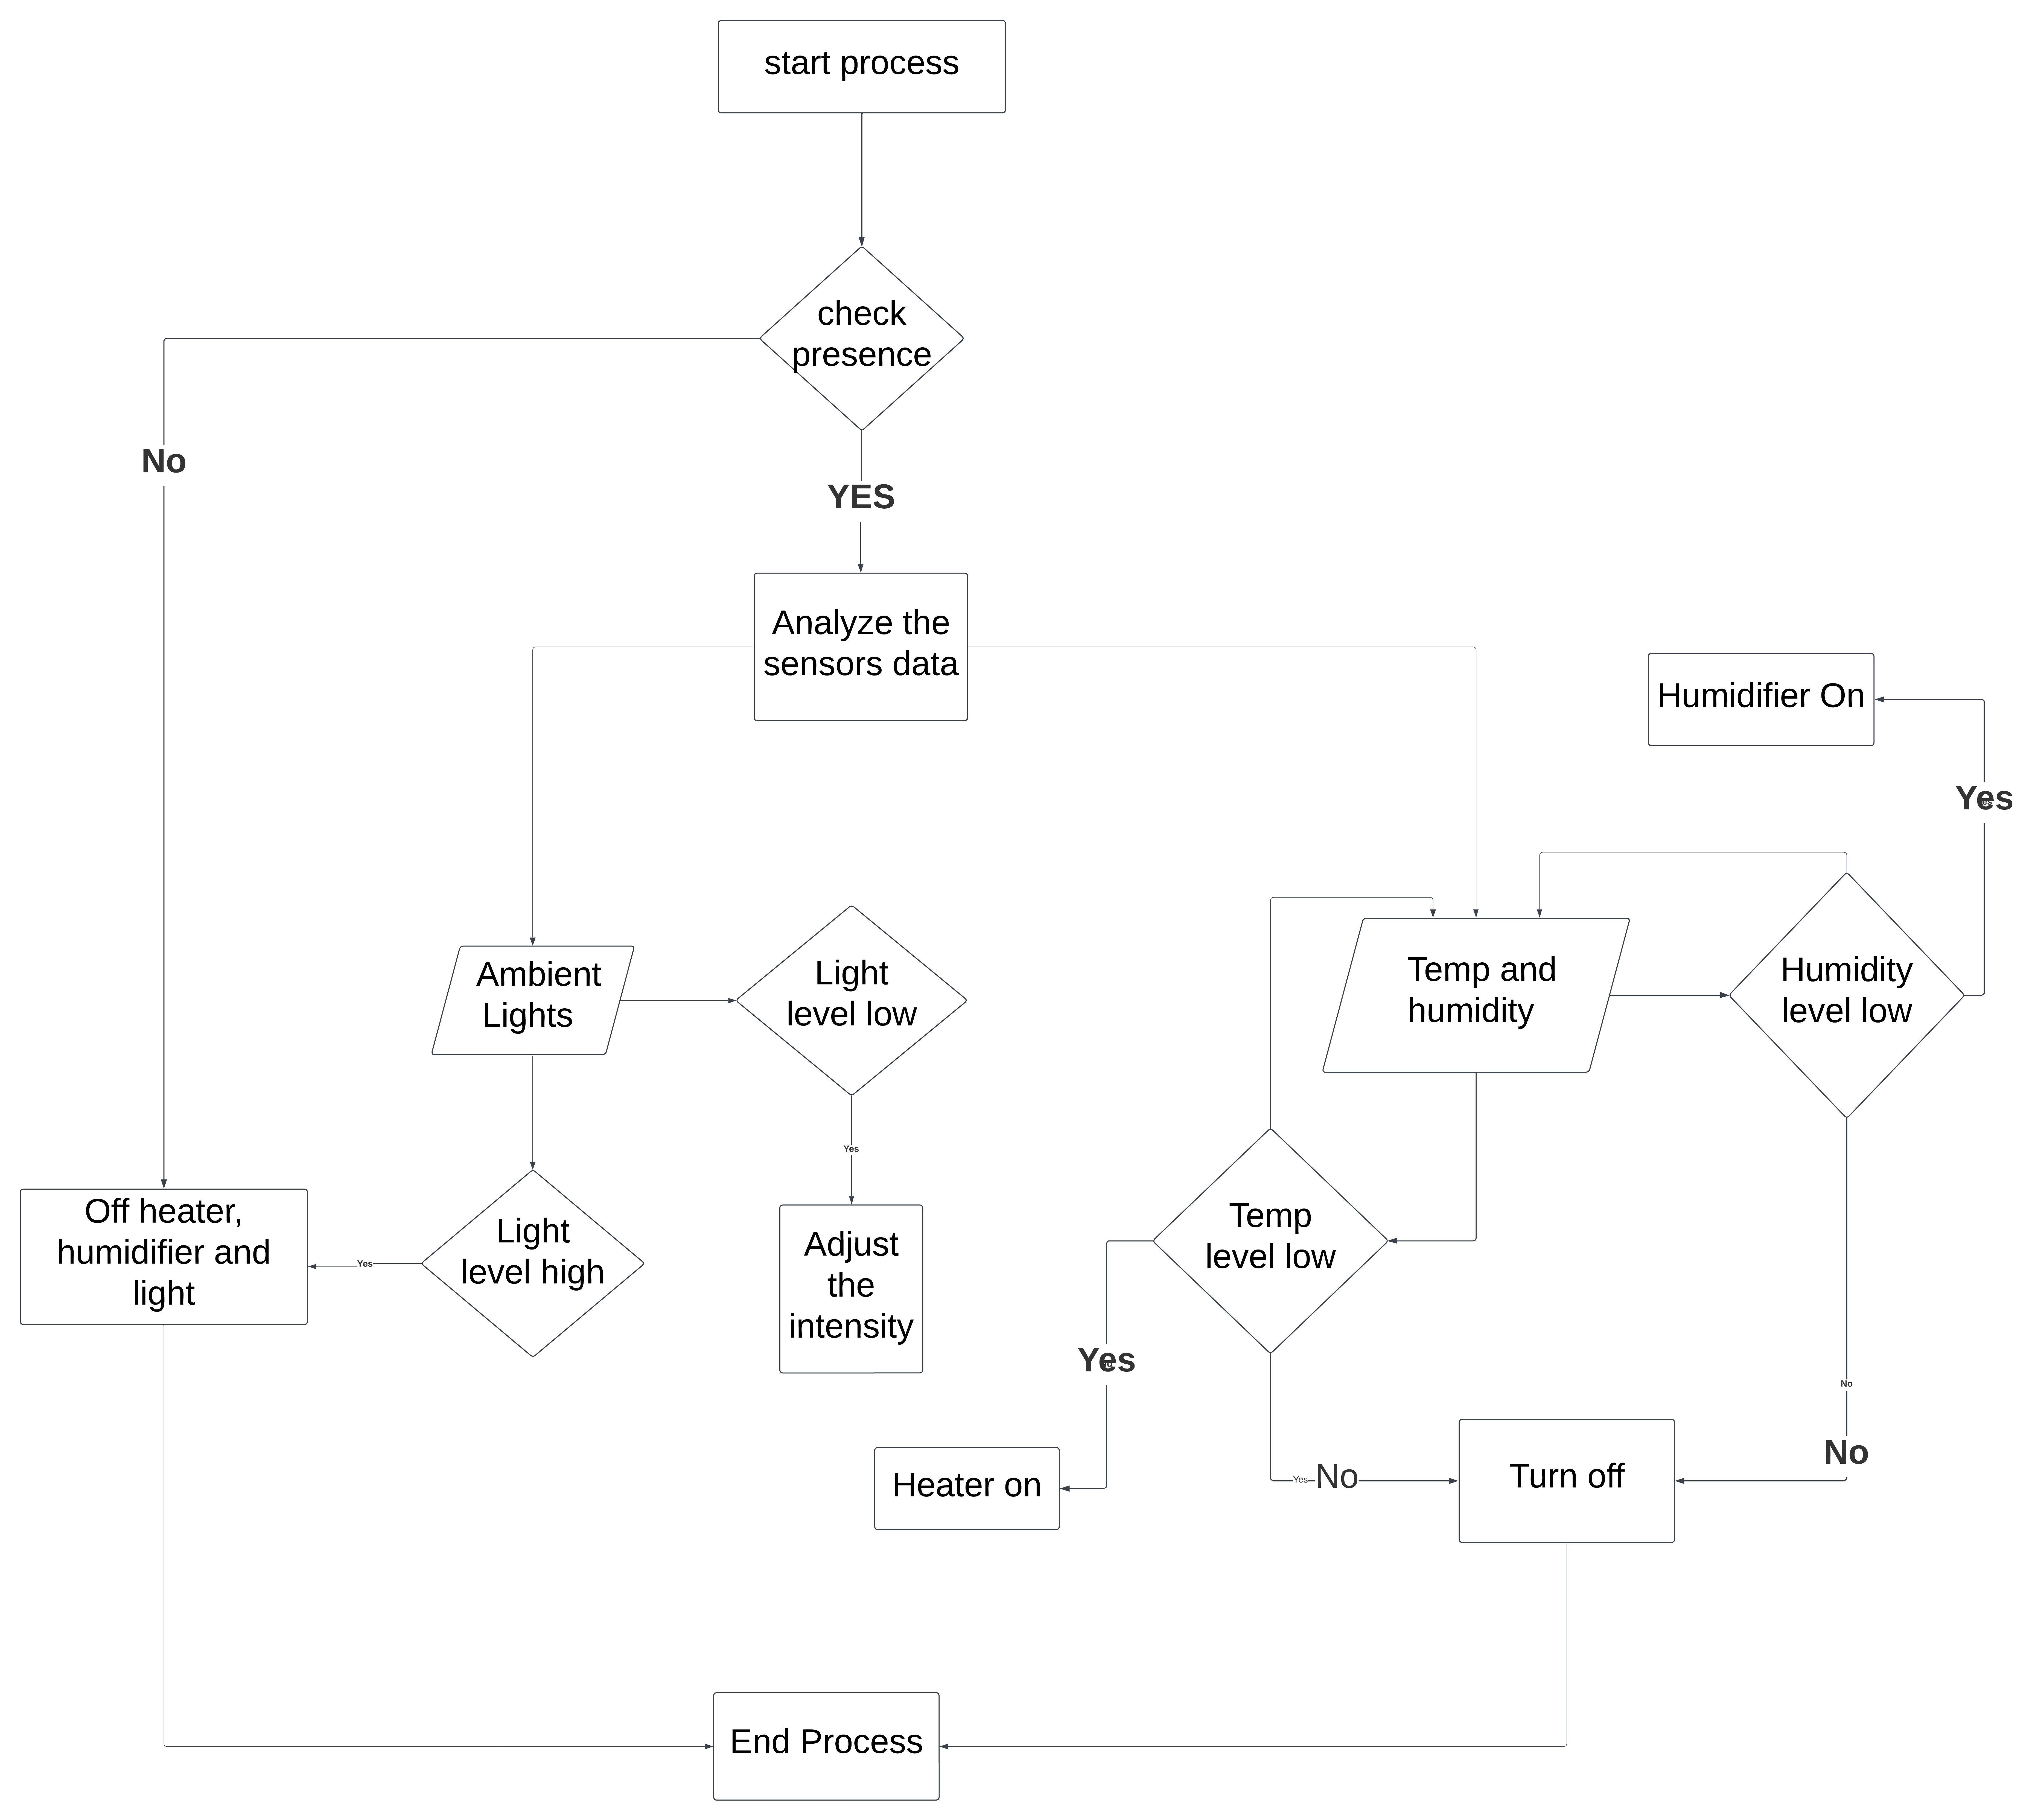
\includegraphics[width=\linewidth]{flowChart.png}
		\caption{Flowchart of the system}
		\label{fig:my_label}
	\end{figure}

	\subsection{Approach}
	A mixed-methods approach will be employed, combining quantitative and qualitative research techniques. The quantitative aspect will focus on testing the system's accuracy, response time, energy efficiency, and the overall effectiveness of the system in maintaining the desired indoor climate. The qualitative approach will gather user feedback on system usability, comfort, and perceived health benefits. By integrating both methods, the study will provide a holistic evaluation of ComfortSphere's functionality and its impact on users' daily lives.

	\subsection{Data Collection and Access}
	The data collection process will involve continuous monitoring of key environmental variables, including temperature, humidity, occupancy, and light intensity. The following sensors will be used in this study:

	\begin{itemize}
		\item \textbf{DHT22 Sensor:} A high-precision sensor used to measure indoor temperature and humidity levels.
		\item \textbf{HC-SR501 PIR Motion Sensor:} A passive infrared sensor used to detect motion and occupancy in the environment.
		\item \textbf{TSL2561 Light Sensor:} A sensor that measures ambient light intensity, which will help regulate lighting conditions.
	\end{itemize}

	These sensors will provide continuous data, which will be logged and transmitted in real-time to the ComfortSphere application via the Pinecone microcontroller.

	\subsection{User Interaction}
	Users will interact with the ComfortSphere system through a dedicated GUI, which allows them to set and adjust climate preferences (temperature, humidity, light), monitor real-time data, and view historical environmental records. Additionally, the GUI will provide users with health-related information, such as how climate adjustments may be benefiting their comfort or health.

	\subsection{User Interaction}
	To assess the user experience, feedback will be gathered through both quantitative surveys and qualitative structured interviews. These will focus on the following areas:
	- System usability: How easy and intuitive the system is to use.
	- Health benefits: Whether users experience noticeable improvements in comfort, especially those with respiratory issues.
	- Overall satisfaction: General user satisfaction with the system's performance and effectiveness in maintaining a comfortable and healthy environment.

	User feedback will be categorized based on three primary user profiles:
	1. \textbf{Health-conscious Users:} Individuals with respiratory conditions such as asthma or COPD, who need precise environmental control to avoid triggering symptoms.
	2. \textbf{Energy-conscious Users:} Homeowners focused on reducing energy consumption and minimizing utility costs through smart climate control.
	3. \textbf{Safety-conscious Users:} Older or vulnerable individuals for whom safety and convenience features (such as automated lighting and motion detection) are most important.

	\subsection{Use Cases and Experiment Selection}
	The experimental evaluation will involve three distinct user groups:
	- \textbf{Health-related Users:} Participants with respiratory difficulties will test how ComfortSphere regulates humidity and temperature to alleviate symptoms. The system's health-oriented features will be particularly important in this group.
	- \textbf{Energy-conscious Users:} This group will evaluate ComfortSphere's effectiveness in reducing energy consumption through adaptive climate control based on occupancy and environmental conditions.
	- \textbf{Safety-conscious Users:} This group, including elderly users, will focus on ComfortSphere's safety features, such as motion detection for lights and energy-efficient environmental control.

	Each user group will engage with the ComfortSphere system for a two-week period. During this time, system performance, energy consumption, and user satisfaction will be closely monitored and compared across the different user profiles.

	\subsection{Time Frame}
	The experimental phase is expected to last for approximately two months, divided as follows:
	- Two weeks for each user group to interact with the system.
	- Four weeks for data analysis, system calibration, and refinement based on user feedback.

	\subsection{Data Recording}
	Sensor data will be collected continuously and stored on the Pinecone microcontroller. The data will be transmitted to a server, which can be accessed through the ComfortSphere application for real-time monitoring. Key data points include:
	- Temperature and humidity levels
	- Motion detection and occupancy
	- Light intensity readings
	- Energy consumption patterns

	\subsection{Data Analysis}
	The quantitative data will be processed using statistical software to analyze trends, variances, and correlations between system performance and user preferences. Specifically, the analysis will focus on:
	- Accuracy and responsiveness of the system in maintaining user-defined climate conditions.
	- Energy efficiency of the system, including reductions in energy consumption through motion-based climate control.
	- Correlations between environmental variables (e.g., temperature, humidity, light) and user satisfaction levels.

	Qualitative data collected from surveys and interviews will be analyzed through thematic coding. Key themes will include:
	- User satisfaction with system usability and performance.
	- Perceived health benefits, especially for users with respiratory conditions.
	- Feedback on energy efficiency and comfort.

	\subsection{Evaluation Metrics}
	The evaluation of ComfortSphere will consider both the quantitative and qualitative metrics:
	- \textbf{System Performance Metrics:} Accuracy of climate control, system responsiveness, energy consumption, and sensor reliability.
	- \textbf{User Satisfaction Metrics:} Usability, perceived health benefits, overall comfort, and general satisfaction, as assessed through surveys and interviews.

	By combining both objective measurements and subjective feedback, this methodology aims to provide a comprehensive understanding of ComfortSphere's performance and its impact on different user groups.
    
    \subsection{Statistical Analysis Plan}
    The statistical analysis of collected data will follow a structured approach to ensure robust and meaningful results. Descriptive statistics, including means, standard deviations, and frequency distributions, will be calculated for all quantitative variables. For continuous environmental data (temperature, humidity, light levels), time-series analysis will be performed to identify patterns, trends, and anomalies. Comparative analysis will be conducted across different user groups to identify variations in system performance and user satisfaction based on specific needs and preferences.
    
    Statistical significance will be assessed using appropriate tests:
    \begin{itemize}
        \item Paired t-tests will compare environmental conditions before and after ComfortSphere implementation.
        \item ANOVA will analyze differences in system performance across the three user groups.
        \item Multiple regression analysis will identify relationships between environmental parameters and user satisfaction metrics.
        \item Chi-square tests will evaluate categorical data from surveys and questionnaires.
    \end{itemize}
    
    All statistical analyses will be performed using R statistical software (version 4.1.2), with a significance level set at p < 0.05. Results will be visualized using appropriate graphs and charts to facilitate interpretation and communication of findings.
    
    \subsection{Ethical Considerations}
    The study will adhere to strict ethical guidelines to protect participant privacy and ensure informed consent. All participants will be provided with detailed information about the study's purpose, procedures, and data collection methods before giving written consent to participate. Personal data will be anonymized, and all information will be stored securely with access restricted to authorized research team members only.
    
    The research protocol has been reviewed and approved by the Institutional Review Board at Schmalkalden University of Applied Sciences (approval number: SUAS-IOT-2024-089). Special considerations will be made for vulnerable participants, such as elderly individuals, ensuring that their participation does not cause any discomfort or inconvenience. Participants will have the right to withdraw from the study at any time without any negative consequences.
    
    \subsection{Pilot Testing}
    Prior to full-scale implementation, a pilot test will be conducted with a small sample of six participants (two from each user group) to validate the experimental protocol, identify potential issues, and refine the data collection instruments. The pilot test will run for one week and will include all aspects of the main study, including sensor setup, data collection, and user feedback mechanisms.
    
    Based on the pilot test results, necessary adjustments will be made to the experimental design, sensor configurations, and survey instruments to ensure optimal performance and data quality during the main study. Feedback from pilot participants regarding system usability and interface design will be particularly valuable in refining the ComfortSphere application before full-scale deployment.

	\section{Hardware Setup}
	\label{sec:hardware setup}
	The hardware setup for the ComfortSphere system is designed to integrate various sensors and actuators to control and monitor indoor climate conditions effectively. The system is based on an IoT framework, utilizing a combination of precise sensors, a microcontroller, and the necessary components to interface with the ComfortSphere application. 

	The key hardware components of the system are as follows:

	\begin{itemize}
		\item \textbf{Pinecone Microcontroller:} The central processing unit of the ComfortSphere system, responsible for collecting data from sensors, processing the information, and communicating with the server and user application. The microcontroller ensures real-time data transmission and system responsiveness.
		\item \textbf{DHT22 Sensor:} This sensor measures both temperature and humidity with high accuracy. It is used to regulate indoor climate conditions based on user preferences for temperature and humidity control.
		\item \textbf{HC-SR501 PIR Motion Sensor:} This sensor detects motion and occupancy in a room. It plays a key role in adaptive climate control by adjusting temperature, humidity, and lighting based on the detected presence of users.
		\item \textbf{TSL2561 Light Sensor:} The TSL2561 measures ambient light intensity, enabling the system to automatically adjust indoor lighting according to natural light levels, promoting energy efficiency and user comfort.
		\item \textbf{Relay Modules and Actuators:} These components are used to control HVAC systems (heaters, humidifiers) and lighting, responding to the sensor data and user preferences. The relays are activated through the microcontroller to implement automated climate and lighting adjustments.
	\end{itemize}

	The sensors are connected to the Pinecone microcontroller, which processes the collected data and sends it to the ComfortSphere application via a server. The system can adjust environmental settings dynamically, providing a responsive and comfortable living experience for the user. Additionally, the platform allows users to interact with the system remotely via a GUI, giving them control over their indoor environment.

	This hardware setup facilitates seamless communication between the sensors and the actuators, ensuring that the system continuously adapts to changing environmental conditions and user needs.
    
    \subsection{Component Specifications and Selection Criteria}
    Each hardware component in the ComfortSphere system was selected based on specific criteria to ensure optimal performance, reliability, and compatibility. The detailed specifications and selection rationale for key components are as follows:
    
    \subsubsection{Pinecone Microcontroller}
    The Pinecone microcontroller was selected as the central processing unit for ComfortSphere based on its balanced combination of processing power, energy efficiency, and connectivity options. Key specifications include:
\begin{itemize}
    \item Processor: 32-bit ARM Cortex-M4 running at 120 MHz
    \item Memory: 256 KB SRAM and 1 MB Flash storage
    \item Connectivity: Built-in Wi-Fi (802.11b/g/n), Bluetooth 5.0, and multiple GPIO pins
    \item Power Consumption: 80mA active mode, 10~\textmu A sleep mode
    \item I/O Capabilities: 12 analog inputs, 24 digital I/O pins, I2C, SPI, and UART interfaces
\end{itemize}

    
    These specifications enable the microcontroller to process sensor data in real-time while maintaining low power consumption for continuous operation. The built-in connectivity options facilitate seamless communication with both sensors and cloud services, eliminating the need for additional modules and reducing system complexity.
    
    \subsubsection{DHT22 Temperature and Humidity Sensor}
    The DHT22 sensor was selected for its high accuracy and reliability in measuring temperature and humidity. Specifications include:
    \begin{itemize}
        \item Temperature Range: -40°C to 80°C with ±0.5°C accuracy
        \item Humidity Range: 0-100\% RH with ±2\% accuracy
        \item Resolution: Temperature (0.1°C), Humidity (0.1\% RH)
        \item Sampling Rate: Once every 2 seconds
        \item Operating Voltage: 3.3V to 5V DC
        \item Digital signal output for noise immunity
    \end{itemize}
    
    The DHT22 offers superior performance compared to alternatives like the DHT11, particularly in accuracy and range. Its digital output also provides better noise immunity compared to analog sensors, ensuring reliable readings even in environments with electrical interference.
    
    \subsubsection{HC-SR501 PIR Motion Sensor}
    The HC-SR501 was selected for occupancy detection due to its sensitivity, range, and power efficiency:
    \begin{itemize}
        \item Detection Range: Up to 7 meters at a 110° angle
        \item Voltage: 5V-12V input
        \item Output: 3.3V digital signal
        \item Adjustable sensitivity and delay time
        \item Low power consumption: <50μA standby current
        \item Built-in temperature compensation for reliable detection across varying environments
    \end{itemize}
    
    The sensor's adjustable sensitivity and delay settings enable fine-tuning for different room sizes and occupancy patterns, minimizing false positives while ensuring reliable detection.
    
    \subsubsection{TSL2561 Light Sensor}
    The TSL2561 light sensor was chosen for its wide dynamic range and spectral response similar to the human eye:
    \begin{itemize}
        \item Dynamic Range: 0.1 to 40,000 Lux
        \item Spectral Response: Close to human eye response
        \item Interface: I2C digital interface
        \item Power Consumption: 0.5mA active, <15μA power down
        \item Programmable interrupt function
        \item 16-bit resolution
    \end{itemize}
    
    Unlike simple photoresistors, the TSL2561 provides accurate lux measurements across a wide range of lighting conditions and features built-in infrared filtering, making it ideal for adaptive lighting control.
    
    \subsubsection{Relay Modules}
    The system uses 5V relays with the following specifications:
    \begin{itemize}
        \item Operating Voltage: 5V DC
        \item Current Rating: 10A at 250VAC or 30VDC
        \item Isolation: Optocoupler isolation between control and switching circuits
        \item Switching Time: <10ms
        \item Indicators: LED status indicators for each relay
    \end{itemize}
    
    These relays provide reliable switching for connected appliances while ensuring electrical isolation between the low-voltage control circuitry and high-voltage appliances.
    
    \subsection{Hardware Integration and Assembly}
    The physical integration of ComfortSphere components follows a modular approach to facilitate installation, maintenance, and future upgrades. The system is housed in a compact enclosure (dimensions: 150mm × 120mm × 45mm) with appropriate ventilation to prevent overheating. Internal components are organized into functional modules:
    
    \begin{itemize}
        \item \textbf{Control Module}: Contains the Pinecone microcontroller and power management circuitry
        \item \textbf{Sensor Module}: Houses the DHT22 and TSL2561 sensors with appropriate shielding
        \item \textbf{Relay Module}: Contains the relay array and driver circuitry
        \item \textbf{Power Supply}: Provides regulated power to all components
    \end{itemize}
    
    The modular design allows for easy replacement of individual components and facilitates system expansion through additional sensor or actuator modules. All connections between modules use standardized connectors, eliminating the need for soldering during maintenance or upgrades.
    
    \subsection{Power Management}
    The ComfortSphere system incorporates a comprehensive power management strategy to ensure reliable operation while minimizing energy consumption:
    
    \begin{itemize}
        \item \textbf{Main Power}: The system operates from a 5V DC power adapter with overcurrent and overvoltage protection.
        \item \textbf{Backup Power}: A 3000mAh LiPo battery provides backup power during outages, enabling up to 24 hours of continued operation of essential functions.
        \item \textbf{Power Optimization}: Dynamic power management reduces consumption during periods of inactivity by selectively disabling non-essential components and utilizing low-power modes of the microcontroller.
        \item \textbf{Voltage Regulation}: Dedicated low-dropout regulators provide clean power to sensitive components, ensuring accurate sensor readings and reliable microcontroller operation.
    \end{itemize}
    
    This power management approach ensures that ComfortSphere operates reliably while minimizing its own energy footprint, aligning with the system's broader energy efficiency goals.
    
    \subsection{Hardware Testing and Calibration}
    Prior to deployment, each ComfortSphere unit undergoes comprehensive testing and calibration to ensure accuracy and reliability:
    
    \begin{itemize}
        \item \textbf{Sensor Calibration}: All sensors are calibrated against reference instruments to ensure measurement accuracy. The DHT22 is calibrated using a NIST-traceable hygrometer and thermometer, while the TSL2561 is calibrated using a professional light meter.
        \item \textbf{System Integration Testing}: The complete system undergoes integrated testing to verify correct communication between components and appropriate response to environmental changes.
        \item \textbf{Stress Testing}: Each unit is subjected to extended operation under varying conditions to identify potential reliability issues before deployment.
        \item \textbf{Power Cycling}: Multiple power cycle tests ensure that the system recovers properly from power interruptions and continues to function as expected.
    \end{itemize}
    
    These rigorous testing procedures ensure that each ComfortSphere unit meets performance specifications and will provide reliable service throughout its operational life.

	\section{Implementation and Software Design}
	\label{sec:implementation}
	The implementation of ComfortSphere encompasses both firmware running on the Pinecone microcontroller and software components operating in the cloud and on user devices. This section details the software architecture, algorithms, and user interface design that enable ComfortSphere's intelligent environmental control capabilities.
	
\subsection{Firmware Architecture}
The firmware running on the Pinecone microcontroller is the backbone of ComfortSphere's real-time environmental monitoring and control. It is built on a real-time operating system (RTOS) to ensure efficient task management and responsiveness. The firmware is structured into several key components, each responsible for specific functionalities:

\begin{itemize}
	\item \textbf{Sensor Management Module:} This module handles the integration and communication with all connected sensors, including the \texttt{DHT22} temperature and humidity sensor, the \texttt{HC-SR501 PIR} motion sensor, and the \texttt{TSL2561} light sensor. It ensures that data is collected at regular intervals and transmitted to the data processing module.
	\item \textbf{Data Processing Module:} This module processes raw sensor data, applying calibration and filtering algorithms to ensure accuracy. It also performs preliminary analysis, such as detecting occupancy patterns or identifying anomalies in environmental conditions.
	\item \textbf{Control Logic Module:} This module implements the core algorithms for environmental control. It uses processed sensor data to make decisions, such as adjusting the HVAC system or dimming lights based on occupancy and ambient conditions.
	\item \textbf{Communication Module:} This module facilitates communication between the microcontroller and external systems, such as the cloud backend and user devices. It supports protocols like MQTT and HTTP for seamless data exchange.
	\item \textbf{Power Management Module:} To optimize energy consumption, this module manages the power states of the microcontroller and connected peripherals, ensuring that the system operates efficiently even in low-power modes.
\end{itemize}

The firmware is designed to be highly configurable, allowing for future upgrades and the integration of additional sensors or actuators. It also includes robust error-handling mechanisms to ensure system reliability.

\section{Findings / Results (Preliminary)}
Since ComfortSphere is in the development phase, the results presented here are based on early-stage testing, integration, and initial sensor performance. The following preliminary observations have been made:

\subsection{Sensor Integration and Testing}  
So far, we have successfully integrated the \texttt{DHT22} temperature and humidity sensors and the \texttt{HC-SR501 PIR} motion sensors into the ComfortSphere system. These sensors have been tested individually and are performing as expected. The \texttt{DHT22} sensor provides accurate temperature readings with a tolerance of $\pm$0.5°C and humidity levels within $\pm$3\%. The \texttt{HC-SR501 PIR sensor} successfully detects motion, triggering necessary adjustments in temperature and humidity. Initial tests indicate that the system can detect occupancy with a response time of less than 2 seconds, ensuring timely adjustments to the environment.

\subsection{Light Sensor Development}  
Work is still ongoing with the \texttt{TSL2561} light intensity sensor. Initial testing has been promising, but we are still refining the sensor's integration and calibration. The goal is to fine-tune the light sensor to adjust the lighting automatically based on ambient light levels. We are currently focusing on ensuring the sensor accurately measures light intensity in a variety of lighting conditions, including low-light and high-glare scenarios. Preliminary results show that the sensor can detect light levels ranging from 0.1 lux to 40,000 lux, but further calibration is needed to improve accuracy in dynamic lighting environments.

\subsection{System Response and Adjustments}  
Although the full system has not yet been tested in a real-world setting, we have simulated environmental adjustments with the current sensors. The system can adjust temperature and humidity based on occupancy detected by the PIR sensor, optimizing the environment when rooms are unoccupied. For example, when no motion is detected for a predefined period, the system reduces heating or cooling by 2-3°C and lowers humidity levels by 5-10\%. This preliminary functionality has been successfully tested in lab environments and will be expanded as additional sensors are fully integrated.

\subsection{Frontend Development Status}  
The frontend development has not yet started. The current focus is on sensor calibration and ensuring the backend is fully functional. Once the sensors are fine-tuned, the team will shift to frontend development, where the app will be designed to offer user-friendly control over system settings, such as temperature, humidity, and lighting. The frontend will also include features for real-time monitoring, historical data visualization, and personalized settings based on user preferences.

\section{Interpretation / Discussion (Preliminary)}
Based on the current stage of ComfortSphere’s development, we can provide preliminary insights and discuss the expected benefits and challenges:

\subsection{Challenges & Limitations}
Sensor Reliability & Calibration
Sensors like DHT22 and HC-SR501 may be accuracy-limited to require periodic calibration.
Environmental factors (e.g., windows, HVAC registers nearby) may impact sensor output.
Compatibility & Integration Issues
Need to integrate seamlessly with current smart home ecosystems (Alexa, Google Home, Apple HomeKit).
Some homes may lack the infrastructure needed for automation.
Cost & Adoption Barriers
High-end multi-sensor systems may be expensive, limiting adoption by price-sensitive consumers.
Non-smart home users might encounter difficulty in setup and use.

\subsection{Key Differentiators}
Smart Adaptation: Traditional HVAC systems are based on pre-programmed schedules or manual adjustments, while ComfortSphere adapts dynamically to the real environmental conditions.
Health-Conscious Design: Unlike traditional systems, ComfortSphere takes into account humidity, air quality, and occupant presence to design a healthier indoor environment.
Energy Efficiency: By switching off or adjusting settings when rooms are unoccupied, it significantly reduces electricity charges and carbon footprint.

\subsection{Sensor Performance and Integration}  
The integration of temperature and humidity sensors has gone smoothly, and we expect that the system’s environmental control will be highly effective once the light sensor integration is complete. The motion detection feature is expected to enhance energy efficiency by ensuring that the system only adjusts the environment when rooms are occupied. This will help reduce energy usage and contribute to sustainable living, even before the system's full functionality is realized. The system's ability to detect occupancy and adjust environmental conditions in real-time is a significant step toward creating a responsive and energy-efficient smart home ecosystem.

\subsection{Challenges with Light Sensor Calibration}  
One of the key challenges we are currently addressing is the calibration of the \texttt{TSL2561} light sensor. The sensor's ability to accurately measure light intensity and adjust the lighting in real-time is crucial to the success of the system. We are focused on ensuring that the sensor provides accurate readings across various lighting conditions (e.g., daylight, artificial lighting, night) to allow for precise control. Further testing will help refine its response to dynamic changes in light levels. For instance, we are experimenting with adaptive algorithms that account for sudden changes in light, such as curtains being opened or closed, to ensure smooth transitions in lighting adjustments.

\subsection{Energy Efficiency and Sustainability}  
The initial findings suggest that ComfortSphere has the potential to optimize energy use significantly by adjusting environmental conditions (temperature, humidity, lighting) based on occupancy. The integration of motion detection ensures that energy is not wasted in unoccupied spaces, a feature that will contribute to lowering energy consumption and promoting a sustainable living environment. As the light sensor becomes fully operational, we expect that ComfortSphere will further enhance its energy-saving potential by controlling both heating and lighting in response to environmental needs. For example, the system could reduce lighting intensity during daylight hours or turn off lights entirely in unoccupied rooms, further reducing energy consumption.

\subsection{Frontend Development and User Experience}  
Although frontend development has not yet started, the design will focus on ease of use and customization. The app will provide users with intuitive control over environmental settings, including adjusting the temperature, humidity, and light intensity according to their preferences. User feedback will be crucial in shaping the final design, and we plan to incorporate features that allow for real-time monitoring and easy adjustments. For instance, users will be able to set schedules for environmental adjustments or receive notifications when the system detects unusual conditions, such as a sudden drop in temperature or a spike in humidity.

\subsection{Future Directions}  
As we continue to work on integrating the light sensor, testing in real environments will become essential. This will provide data on the system’s real-world performance and its ability to adapt to varied conditions. Once the frontend is developed, user trials will help refine the system’s features and functionality. Additionally, as ComfortSphere evolves, AI-driven algorithms may be introduced to predict user preferences and automate environmental adjustments based on historical patterns. For example, the system could learn a user's preferred temperature and lighting settings at different times of the day and automatically adjust the environment accordingly. Future iterations may also include integration with other smart home devices, such as smart blinds or air purifiers, to create a fully interconnected ecosystem.

\section{Conclusion}
\label{sec:conclusion}
In this paper, we presented ComfortSphere, an IoT-enabled smart home system designed to provide automated, adaptive climate control to enhance user comfort, energy efficiency, and health. The system integrates a range of sensors, including temperature, humidity, motion, and light sensors, to monitor and adjust the indoor environment dynamically. By using the Pinecone microcontroller, ComfortSphere can collect real-time data, process it, and control actuators such as HVAC systems and lighting to create a personalized living space for users.

The experimental setup, involving health-conscious, energy-conscious, and safety-conscious users, will provide insights into the system's accuracy, efficiency, and overall performance. The results of the user feedback and sensor data analysis will inform further improvements and refinements to the system. ComfortSphere holds the potential to meet the growing demand for smart home systems that not only optimize energy consumption but also prioritize the health and well-being of users.

Future work will focus on enhancing the system's adaptability and refining the user interface to ensure ease of use for all user categories. Ultimately, ComfortSphere aims to contribute to the development of smart home technologies that foster sustainable living while improving quality of life. By combining advanced sensor technology, intelligent algorithms, and user-centric design, ComfortSphere represents a significant step forward in the evolution of smart home systems.

	\printbibliography[title={References}]
\end{document}